%!TEX root = emnlp2016.tex

In this section we develop the Capsule model for detecting and characterizing events.  Capsule relies on text data sent between entities over time, and builds on topics models. We first give the intuition on Capsule, then formally specify the model.  We also describe how to explore a corpus using Capsule and how we learn its hidden variables.

\begin{figure}
\centering
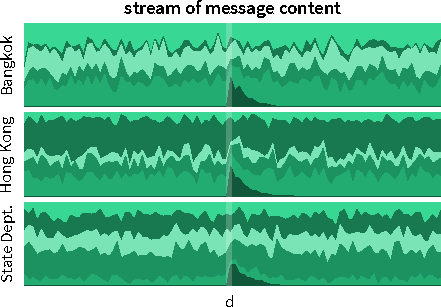
\includegraphics[width=\linewidth]{fig/cartoon.pdf}
\caption{Cartoon intuition of Capsule; the $y$ axis is the stacked proportion of messages about various subjects during a given time interval.  The Bangkok embassy, Honk Kong embassy, and State Department all have typical concerns about which they usually send messages.  When an events occurs at time $t$, the stream of message content alters to include the event, then fades back to ``business as usual.''  Capsule discovers entities' typical concerns as well as the event occurrence and content.}
\label{fig:cartoon}
\end{figure}

Consider an entity like the Bangkok American embassy, shown in Figure~\ref{fig:cartoon}.  We can imagine that there is a stream of messages (or \emph{diplomatic cables}) being sent by this embassy---some might be sent to the US State Department, others to another American embassy like Hong Kong.  An entity will usually talk about certain topics; the Bangkok embassy, for instance, is concerned with topics regarding southeast Asia more generally.

Now imagine that at a particular time $t$, an event occurs, such as the capture of Saigon during the Vietnam war.  We do not directly observe that events occur, but we do observe the message stream.  Using this stream, each event will be described as a distribution over the vocabulary, similar to how topics are distributions over these same terms.  When an event occurs, the message content changes for multiple entities---significant events impact multiple parties simultaneously. The day following the capture of Saigon, for instance, the majority of the diplomatic cables sent by the Bangkok embassy and several other entities were about Vietnam war refugees.
Thus we imagine that an entity's stream of messages is controlled by what it usually talks about as well as the higher level stream of unobserved events.

% \parhead{Background: Topic Models.} Capsule builds on topic models.  Topic models are algorithms for discovering the main themes in a large collection of documents; each document can then be summarized in terms of the global themes.  More formally, a topic $k$ is a probability distribution over the set of vocabulary words.  Each document $d$ is represented as a distribution over topics $\theta_d$.  Thus we can imagine that when we generate a document, we first pick which topics are relevant (and in what proportions).  Under the LDA topic model~\cite{Blei:2003}, we know the number of words in each document.  Then, for each word, we select a single topic from this distribution over topics, and finally select a vocabulary term from the corresponding topic's distribution over the vocabulary.  Alternatively, we can cast topic modeling as factorization, such as in Poisson factorization~\cite{Gopalan:2014b}, and draw a word count for each term in the vocabulary.

% Topic models are often applied to provide a structure for an otherwise unstructured collection of documents.  Documents, however, are often accompanied by metadata, such as the date written or author attribution; this information is not exploited by traditional topic models.  The Capsule model uses both author and date information to identify and characterize events that influence the content of the collection.

\parhead{Model Specification.}
We now define Capsule in detail. Our data are \textit{entities}
sending \textit{messages} over \textit{time}. The observed variables
are $w_{d,v}$, the number of times term $v$ occurs in message $d$. The
message is associated with an entity (or author) $a_d$ and a time (or
date) interval $i_d$.

We model each message with a bank of Poisson distributions, one per
term in the vocabulary, $w_{d,v} \sim \textrm{Poisson}(\lambda_{d,v})$.
The rate $\lambda_{d,v}$ blends the different influences on the
content of the message, which are defined in terms of different types
of \textit{topics}. A topic, as in typical topic modeling~\cite{Blei:2003,canny2004gap,Gopalan:2014b}, is
a distribution over terms.

Specifically, the message blends general topics about diplomacy (e.g.,
diplomats, communication) $\beta_k$, an entity topic that is specific
to the author of the message (e.g., terms about France) $\eta_{a_d}$,\footnote{These entity-specific topics are similar to background topics~\cite{paul2012model}.}
and an event topic that is specific to the events of relevant recent weeks (e.g.,
terms about an international crisis) $\pi_t$. Notice how messages
share these topics in different configurations: all messages share the
general topics; messages from the same entity share the entity topics;
and messages from the same interval share the event topics.

\begin{table}
\centering
\small
\begin{tabular}{cc}
\toprule
topic type & top terms \\
\midrule
general & plan, visit, arrival, itinerary, visitor\\
entity & soviet, moscow, embasy, ussr, meet \\
event & vietnam, evacuation, evacuate, missionary \\
\bottomrule
\end{tabular}
\label{tab:3topics}
\caption{Top vocabulary terms for examples of each of the three topic varieties; these three types of topics blend to form the distribution of each message.  They come from the model fit we discuss in \Cref{sec:eval}.}
\end{table}

Examples of these three types of topics are in \Cref{tab:3topics}---the general topic 
relates to planning travel, the entity topic captures words related to the U.S.S.R., and 
the event topic captures words related to the evacuation of Saigon toward the end of the Vietnam War.

Each message blends its corresponding topics with different
strengths, which are drawn per message. Each message represents a
different mix of the events of recent weeks, entity-specific items, and
general diplomacy.

Putting this together, the Poisson rate for term $v$ in document $d$ is
\begin{align}
  \lambda_{d,v} = \theta_d^\top\beta_v  + \zeta_d \eta_{a_d,v} + \sum_{t=1}^T f(i_d, t) \epsilon_{d,t} \pi_{t,v},
\label{eq:poisrate}
\end{align} where $\theta_d$ corresponds to strength of general diplomacy, $\zeta_d$ corresponds to strength of entity-specific concerns, and $\epsilon_d$ corresponds to strength of events; $f$ is some function of decay.  This function is important because events should not remain at their full strength indefinitely, but should decay over time.  In our experiments, we find that exponential decay, as in \Cref{eq:f}, performs well.

We place gamma priors on the topic strengths and Dirichlet priors on
the topics. The distributions of general and entity topic strengths are defined
hierarchically by entity, capturing the different topics that each
entity tends to discuss.  The prior on the entity strength is
also defined hierarchically; different weeks are more or less
``eventful.'' The full generative process is in \Cref{fig:generative-model}.

Given a collection of messages, posterior inference uncovers the
different types of topics and how each message exhibits them. We will
see below, how inferences about the event strengths enable us to
filter the corpus to find important messages.

%%%%%%
% As in topic modeling, we represent the general topics of conversation with a $K\times V$ matrix $\beta$, where $K$ is a low dimensional number of topics that we wish to capture, and $V$ is the size of our vocabulary; each row $\beta_k$ is normalized such that it represents the probability of seeing vocabulary word $v$ when discussing topic $k$.  As a generative process, we draw these general topics from a Dirichlet distribution, or $\beta_k \sim \mbox{Dirichlet}_V (\alpha_\beta).$ 

% In addition to using these general topics to represent entity concerns, each entity $n$ has its own exclusive topic $\beta^{(n)}_{0}$, which can be appended as a bias row to the general topics $\beta$.  These entity-specific topics are drawn from a Dirichlet, just as the general topics, and are similar to
% background topics~\cite{paul2012model}.  Without these entity topics, entity-specific stop words (e.g. ``Parisian'' for the Paris embassy) would dominate the general topics.

% The concerns of author $n$ are represented with $\phi_n$, a $(K+1)$-dimensional topic vector, where each element is drawn from a gamma distribution, or $\phi_{n,k} \sim \mbox{Gamma}(s_\phi, r_\phi),$\footnote{We use the shape-rate parameterization for all Gamma distributions.} and the first element of the concern vector $\phi_{n,0}$ describes how much the entity $n$ relies on its exclusive topic $\beta^{(n)}_0$

% Similar to topic modeling, we represent the contents of each document in topic space; each document $d$ has a $(K+1)$-dimensional latent parameter $\theta_d$ to describe the particular contents of that document.  Unlike traditional topic models, each document $d$'s topics depend on the concerns of the author $a_d$; each document topic $\theta_{d,k}$ is drawn from a gamma distribution parameterized by the corresponding author concerns $\phi_{a_d,k}$: $\theta_{d,k} \sim \mbox{Gamma}(s_\theta, \phi_{a_d,k})$.

% To represent events, we consider discrete intervals of time.  Each interval $t$ has a corresponding interval strength $\psi_t$ and description $\pi_t$.  Event strengths are a single value for each interval $t$, and are drawn from a gamma distribution: $\psi_{n,k} \sim \mbox{Gamma}(s_\psi, r_\psi)$.  These strengths indicate how important the interval is in determining message content.  Interval descriptions are similar to topics: each description is a $V$-dimensional vector drawn from a Dirichlet distribution over the vocabulary terms, or $\pi_k \sim \mbox{Dirichlet}_V (\alpha_\pi).$

% Just as we describe each document $d$ in terms of relevant topics with the $\theta_d$ parameters, we also describe the relevancy of each time interval with the $\epsilon_d$ parameters.  These interval relevancy parameters are drawn from gamma distributions and depend on the overall strength $\psi$ of the corresponding interval; for interval $t$ and document $d$ (written at time $i_d$), we have $\epsilon_{d,t} \sim \mbox{Gamma}(s_\epsilon, \psi_{i_d,t})$.

% Conditional on the hidden variables and the author and time metadata, Capsule is a model of how document word counts came to be.  For document $d$ and vocabulary term $v$, we generate the word counts form a Poisson distribution parameterized by the documents topics $\theta_d$ and relevant events $\epsilon$, as well as global topic $\beta$ and event descriptions $\pi$:
% \begin{equation}
% w_{d,v} \sim \mbox{Poisson}\left(\theta_d^\top\beta^{(a_d)}_v + \sum_{t=1}^T f(i_d, t) \epsilon_{d,t} \pi_{t,v}\right),
% \label{eq:generateData}
% \end{equation}
% where $f$ is some function of decay.  This function is important because events should not remain at their full strength indefinitely, but should decay over time.  In our experiments, we consider step functions, linear decay, and exponential decay.  Figure~\ref{fig:generative-model} gives the full generative process for Capsule.


\begin{figure}[htb]
\begin{mdframed}
\small
\begin{itemize}[leftmargin=*]
\item for each time step $t=$~1:$T$,
	\begin{itemize}[leftmargin=*]
	\item draw interval description over vocabulary \\(event topic) $\pi_t \sim \mbox{Dirichlet}_V (\alpha)$
	\item draw interval strength \\$\psi_{t} \sim \mbox{Gamma}(s_\psi, r_\psi)$
	\end{itemize}
\item for each entity $n=$~1:$N$,
	\begin{itemize}[leftmargin=*]
	\item draw entity-specific topics over vocabulary \\$\eta_n \sim \mbox{Dirichlet}_V (\alpha)$
	\item draw entity-specific topic strength \\$\xi_{n} \sim \mbox{Gamma}(s_\xi, r_\xi)$
	\end{itemize}
\item for each topic $k=$~1:$K$,
	\begin{itemize}[leftmargin=*]
	\item draw general topic distribution over vocabulary \\$\beta_k \sim \mbox{Dirichlet}_V (\alpha)$
	\item for each entity $n=$~1:$N$,
		\begin{itemize}[leftmargin=*]
		\item draw general entity concern \\$\phi_{n,k} \sim \mbox{Gamma}(s_\phi, r_\phi)$
		\end{itemize}
	\end{itemize}
\item for each document $d=$~1:$D$ sent at time $i_d$ by author $a_d$,
	\begin{itemize}[leftmargin=*]
	\item draw local entity concern \\$\zeta_{d} \sim \mbox{Gamma}(s_\zeta, \xi_{a_d})$
	\item for each topic $k=$~1:$K$,
		\begin{itemize}[leftmargin=*]
			\item draw local entity concern \\$\theta_{d,k} \sim \mbox{Gamma}(s_\theta, \phi_{a_d,k})$
		\end{itemize}
	\item for each time $t=$~1:$T$,
		\begin{itemize}[leftmargin=*]
			\item draw local interval relevancy \\$\epsilon_{d,t} \sim \mbox{Gamma}(s_\epsilon, \psi_{i_d,t})$ 
		\end{itemize}
	\item for each vocabulary term $v=$~1:$V$,
		\begin{itemize}[leftmargin=*]
			\item set $\lambda_{d,v} = \\ \theta_d^\top\beta_v  + \zeta_d \eta_{a_d} + \sum_{t=1}^T f(i_d, t) \epsilon_{d,t} \pi_{t,v}$
			\item draw word counts $w_{d,v} \sim \mbox{Poisson}\left(\lambda_{d,v}\right)$
		\end{itemize}
	\end{itemize}
\end{itemize}
\end{mdframed}
\caption{The generative process for Capsule.}
\label{fig:generative-model}
\end{figure}


\parhead{Detecting and characterizing events.} 
Once we estimate the posterior distribution of the Capsule parameters, we can use the expectations of the latent parameters to explore the original data.  To detect events, we average the per-document event relevancy parameters $\epsilon$ for each document in the interval and multiply it by the interval strength $\psi$:
\begin{equation}
m_t = \E[\psi_t] \frac{1}{\vert D_t \vert} \sum_{d \in D_t} \E[\epsilon_{d,t},]
\label{eq:eventness}
\end{equation}
where $D_t$ is the set of all cables sent in interval $t$. This measure of ``eventness'' provides a scaled estimate of the number of words that are related to an real-world event in that interval.  Figure~\ref{fig:cables_events} shows events detected with this metric.

Given an identified event, we can characterize it in terms of its top terms under $\pi$, but we can also use event relevancy parameters $\epsilon$ to sort documents; Section~\ref{sec:eval} explores relevant documents for events found in the National Archive diplomatic cables data.
In addition to detecting and characterizing events, Capsule can be used to explore entity concerns and the general themes in a given collection.\footnote{Upon publication, we will release code for a pipeline to visualize and explore a corpus, given a Capsule fit.}

There are connections between Capsule and recent work on Poisson
processes. In particular, we can interpret Capsule as a collection of
related discrete time Poisson processes with random intensity
measures. Further, marginalizing out the event strength prior reveals
that word use from one entity can ``excite'' word use in another, which
suggests a close relationship to Hawkes processes~\cite{hawkes1971spectra}.

\parhead{Learning the hidden variables.}
In order to use the Capsule model to explore the observed documents, we must compute the posterior distribution.  Conditional on the observed word counts $w$, our goal is to compute the posterior values of the hidden parameters---general topics $\beta$, entity topics $\eta$, event topics $\pi$, entity concerns $\phi$ (for general topics) and $\xi$ (for their own topic), overall event strengths $\psi$, and document-specific strengths for general topics $\theta$, entity topics $\zeta$, and event topics $\epsilon$.

As for many Bayesian models, the exact posterior for Capsule is not tractable to compute; approximating it is our central statistical and computational problem.  We develop an approximate inference algorithm for Capsule based on variational methods~\cite{jordan1999introduction},\footnote{Source code is available at https://github.com/?????/capsule.} which is detailed in Appendix~\ref{sec:inference}. This algorithm produces a fitted variational distribution which can then be used as a proxy for the true posterior, allowing us to explore a collection of documents with Capsule.  


% \parhead{Visualization.}
% Capsule is a high-level statistical tool. In order to understand and explore its results, a user must scrutinize numerical distributions.
% To make Capsule more accessible, we developed an open source tool for visualizing its results.\footnote{Source code: https://github.com/?????/capsule-viz.}  Our tool creates a navigator of the documents and latent parameters, allowing users to explore events, entities, topics, and the original documents.  Figure~\ref{fig:viz} shows several screenshots of this browsing interface.

% \begin{figure}
% \centering
% 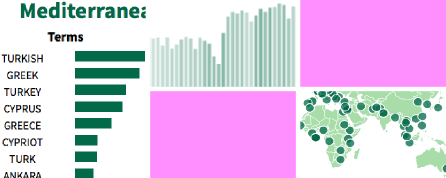
\includegraphics[width=\linewidth]{fig/viz.png}
% \caption{Screenshots of Capsule visualization of US State Department cables.  Left: top words in a topic (manually labeled topic title).  Center-top: events over time (height is volume of messages sent, color is probability of an event occurring).  Center-bottom: topics for an event on <date TODO: cyprus coup?>.  Right-top: cyprus entity topics? TODO.  Right-bottom: entities shown on a map.}
% \label{fig:viz}
% \end{figure}

